 % --------------------------------------------------------------
% Based on a homework template by Dana Ernst (MTH320 Homework
% template on Overleaf).
% --------------------------------------------------------------

\documentclass[12pt]{article}

\usepackage{graphicx}
\graphicspath{{./images/}}
\usepackage[margin=1in]{geometry} 
\usepackage{amsmath,amsthm,amssymb}
% https://tex.stackexchange.com/questions/146306/how-to-make-horizontal-lists
\usepackage[inline]{enumitem} % allows using letters in enumerate list environment
\usepackage[mathscr]{euscript}
% source: https://stackoverflow.com/questions/3175105/inserting-code-in-this-latex-document-with-indentation

\usepackage{listings}
\usepackage{color}
\usepackage{hyperref}

\newtheorem{theorem}{Theorem}

\definecolor{dkgreen}{rgb}{0,0.6,0}
\definecolor{gray}{rgb}{0.5,0.5,0.5}
\definecolor{mauve}{rgb}{0.58,0,0.82}

\lstset{frame=tb,
	language=C, % language for code listing
	aboveskip=3mm,
	belowskip=3mm,
	showstringspaces=false,
	columns=flexible,
	basicstyle={\small\ttfamily},
	numbers=none,
	numberstyle=\tiny\color{gray},
	keywordstyle=\color{blue},
	commentstyle=\color{dkgreen},
	stringstyle=\color{mauve},
	breaklines=true,
	breakatwhitespace=true,
	tabsize=4
}

\newcommand{\N}{\mathbb{N}}
\newcommand{\Z}{\mathbb{Z}}

\newenvironment{ex}[2][Exercise]{\begin{trivlist}
		\item[\hskip \labelsep {\bfseries #1}\hskip \labelsep {\bfseries #2.}]}{\end{trivlist}}

\newenvironment{sol}[1][Solution]{\begin{trivlist}
		\item[\hskip \labelsep {\bfseries #1:}]}{\end{trivlist}}


\begin{document}

% --------------------------------------------------------------
%                         Start here
% --------------------------------------------------------------

\noindent Sergio Garcia Tapia \hfill

\noindent{\small Numerical Linear Algebra, Lloyd Trefethen and David Bau III} \hfill 

\noindent{\small Lecture 4: The Singular Value Decomposition} \hfill 

\noindent\today
\section*{Lecture 4: The Singular Value Decomposition}

\begin{ex}{1}
	Determine SVDs of the following matrices (by hand calculation):
	
	\begin{enumerate*}[label=(\alph*)]
		\item $\begin{bmatrix}
			3 & 0\\
			0 & -2
		\end{bmatrix}$
		\quad\quad
		\item $\begin{bmatrix}
			2 & 0\\
			0 & 3
		\end{bmatrix}$
		\quad \quad
		\item $\begin{bmatrix}
			0 & 2\\
			0 & 0\\
			0 & 0
		\end{bmatrix}$
		\item $\begin{bmatrix}
			1 & 1\\
			0 & 0
		\end{bmatrix}$
		\quad \quad
		\item $\begin{bmatrix}
			1 & 1\\
			1 & 1
		\end{bmatrix}$
	\end{enumerate*}
\end{ex}

\begin{sol}
	\
	\begin{enumerate}[label=(\alph*)]
		\item To determine the SVD, we consider mapping vectors of unit norm to other vectors of unit norm.
		For example, if we let $v_1=e_1$, then $Av_1=3e_1$, so we can set $u_1=e_1$. If we set $v_2=-e_2$,
		then $Av_2=A(-e_2)=2e_2$. Thus we set $u_2 = e_2$. Let $\sigma_1=3$, $\sigma_2=2$. Then define
		$U$ to be the $2\times 2$ matrix whose columns are $u_1$ and $u_2$, $V$ to be the $2\times 2$ matrix
		whose columns are $v_1$ and $v_2$, and $\Sigma$ to be the $2\times 2$ diagonal matrix whose two
		diagonal entries are $\sigma_1$ and $\sigma_2$.
		
		\
		It's easy to see that $U$ and $V$ are unitary because the columns are orthonormal. Note
		\begin{align*}
			U\Sigma V^*e_1 &= U\Sigma e_1=U(3e_1)=3e_1=Ae_1\\
			U\Sigma V^*e_2 &= U\Sigma(-e_2)=U(-2e_2)=-2e_2=Ae_2
		\end{align*}
		Since every vector can be expressed in terms of the standard basis vectors, We conclude that $A=U\Sigma V^*$.
		\item Let $u_1=v_1=v_1$, $u_2=v_2=e_2$, and $\sigma_1=2$, $\sigma_2=3$. If $U$ matrix whose columns
		are $u_1$, $u_2$, $V$ is the matrix whose columns are $v_1$ and $v_2$, and $\Sigma$ is the matrix
		whose diagonal entries are $\sigma_1$ and $\sigma_2$, then $A=U\Sigma V^*$.
		\item This time $Ae_1=0$ and $Ae_2=2e_1$. Let $v_1=e_{2, \mathbb{R}^2}$ and $v_2=e_{1,\mathbb{R}^2}$.
		Let $u_1=e_{1,\mathbb{R}^3}$ and $u_2=e_{2, \mathbb{R}^3}$, $u_3=e_{3,\mathbb{R}^3}$,  $\sigma_1 = 2$, and
		$\sigma_2 = 0$. Then $Av_1=2u_1$, and $Av_2=0$. If we let $U$ be the $3\times 2$ matrix with $u_1$,
		$u_2$, and $u_3$ as columns, $V$ be the matrix with $u_1$ and $u_2$ as columns, and $\Sigma$ be the
		diagonal matrix with diagonal entries $\sigma_1$ and $\sigma_2$, then
		\begin{align*}
			U\Sigma V*&=\begin{bmatrix}
				1 & 0 & 0\\
				0 & 1 & 0\\
				0 & 0 & 1
			\end{bmatrix}
			\begin{bmatrix}
				2 & 0\\
				0 & 0\\
				0 & 0
			\end{bmatrix}
			\begin{bmatrix}
				0 & 1\\
				1 & 0
			\end{bmatrix}^*
			e_{1,\mathbb{R}^2}\\
			&=\begin{bmatrix}
				1 & 0 & 0\\
				0 & 1 & 0\\
				0 & 0 & 1
			\end{bmatrix}
			\begin{bmatrix}
				2 & 0\\
				0 & 0\\
				0 & 0
			\end{bmatrix}e_{2,\mathbb{R}^2}\\
			&=0=Ae_{1,\mathbb{R}^2}
		\end{align*}
		and
		\begin{align*}
			U\Sigma V*&=\begin{bmatrix}
				1 & 0 & 0\\
				0 & 1 & 0\\
				0 & 0 & 1
			\end{bmatrix}
			\begin{bmatrix}
				2 & 0\\
				0 & 0\\
				0 & 0
			\end{bmatrix}
			\begin{bmatrix}
				0 & 1\\
				1 & 0
			\end{bmatrix}^*
			e_{2,\mathbb{R}^2}\\
			&=\begin{bmatrix}
				1 & 0 & 0\\
				0 & 1 & 0\\
				0 & 0 & 1
			\end{bmatrix}
			\begin{bmatrix}
				2 & 0\\
				0 & 0\\
				0 & 0
			\end{bmatrix}
			e_{1,\mathbb{R}^2}\\
			&=\begin{bmatrix}
				1 & 0 & 0\\
				0 & 1 & 0\\
				0 & 0 & 1
			\end{bmatrix}
			2e_{1,\mathbb{R}^3}\\
			&=2e_{1\mathbb{R}^3}\\
			&=Ae_{2,\mathbb{R}^2}
		\end{align*}
		Hence $A=U\Sigma V^*$.
		\item Let $v_1=\frac{1}{\sqrt{2}}(e_1 + e_2)$ and $u_1=e_1$ so that $Av_1 = \frac{2}{\sqrt{2}}e_1
		=\frac{2}{\sqrt{2}}u_1$. Let $v_2=\frac{1}{\sqrt{2}}(e_1-e_2)$ and $u_2=e_2$. Then
		$Av_2=0$. Set $\sigma_1=\frac{2}{\sqrt{2}}$, and $\sigma_2=0$. Define $U$ to be the matrix whose
		columns are $u_1$ and $u_2$, $V$ to be the matrix whose columns are $v_1$ and $v_2$, and
		$\Sigma$ to be the diagonal matrix whose diagonal entries are $\sigma_1$ and $\sigma_2$. Then
		\begin{align*}
			U\Sigma V^*e_1=&\Sigma V^*e_1=\Sigma \left(\frac{1}{\sqrt{2}}(e_1+e_2)\right)=\frac{2}{\sqrt{2}}\cdot  \frac{1}{\sqrt{2}}e_1=e_1=Ae_1\\
			U\Sigma V^*e_2&=\Sigma V^*e_2=\Sigma \left(\frac{1}{\sqrt{2}}(e_1-e_2)\right)=\frac{2}{\sqrt{2}}\cdot \frac{1}{\sqrt{2}}e_1=e_1=Ae_2
		\end{align*}
		Hence $A=U\Sigma V^*$.
		\item Let $u_1=v_1=\frac{1}{\sqrt{2}}(e_1+e_2)$, so that $Av_1=\frac{2}{\sqrt{2}}(e_1+e_2)=2u_1$.
		Similarly let $u_2=v_2=\frac{1}{\sqrt{2}}(e_1-e_2)$, so that $Av_2=0$. Define $\sigma_1=2$ and
		$\sigma_2=0$. Then if we let $U$ be the matrix whose columns are $u_1$ and $u_2$, let $V$ be the
		matrix whose columns are $v_1$ and $v_2$, and $\Sigma$ be the diagonal matrix whose diagonal entries
		are $\sigma_1$ and $\sigma_2$, we get $A=U\Sigma V^*$.
	\end{enumerate}
\end{sol}

\begin{ex}{4.2}
	Suppose $A$ is an $m\times n$ matrix and $B$ is the $n\times m$ matrix obtained by rotating $A$
	ninety degrees clockwise on paper (not exactly a standard mathematical transformation!). Do $A$
	and $B$ have the same singular values? Prove that the answer is yes, or give a counter example.
\end{ex}

\begin{sol}
	\
	\begin{proof}
		Suppose $A\in\mathbb{C}^{m\times n}$. Then $B$ and $A^T$ are both $n\times m$, and they
		are mirror images of one another. That is, given row $b_i^*$ of $B$, the entries in the $i$-th row
		of $A^T$ has the same entries listed in the reverse order. As a result, $A^T$ and $B$ contain
		the same columns in reverse. In other words, if we let $J$ be the matrix whose columns are
		$e_n,\ldots,e_1$, meaning the standard basis vectors in reverse, then $B=A^TJ$.
		
		\
		First, note that if $Q$ is unitary, then $Q^T$ is unitary because $(Q^*)^T=(Q^T)^*$, so
		\begin{align*}
			Q^*Q&=I\\
			(Q^*Q)^T&=I^T\\
			Q^T(Q^*)^T&=I
		\end{align*}
		Thus, if $A$ has an singular value decomposition $A=U\Sigma V^*$, then $A^T=(V^*)^T\Sigma^TU^T$, which is a singular value decomposition of
		$A^T$, so
		\begin{align*}
			B &= (V^*)^T\Sigma^T U^TJ\\
			&=(V^*)^T\Sigma^T (J^TU)^T
		\end{align*}
		Since the product of unitary matrices is unitary, we see that $J^TU$ is unitary, and thus
		$(J^TU)^T$ is unitary. Hence the equation above is a singular value decomposition of $B$.
		Since $\Sigma$ is diagonal, its entries are the same as $\Sigma^T$, and hence $A$ and $B$ have
		the same singular values.
	\end{proof}
\end{sol}

\begin{ex}{4.3}
	Write a MATLAB program (see Lecture 9) which, given a real $2\times 2$ matrix $A$, plots the right
	singular vectors $v_1$ and $v_2$ in the unit circle and also the left singular vectors $u_1$ and
	$u_2$ in the appropriate ellipse, as in Figure 4.1. Apply your program to the matrix (3.7) and
	also to the $2\times 2$ matrices of Exercise 4.1.
\end{ex}

\begin{sol}
	\
	I have implemented the program in Python, consisting of the files \texttt{main.py} and
	and \texttt{plot\_singular\_vectors.py} under the directory \texttt{./03-svd-vector-plot}.
	See Figure~\ref{fig:4.3-eq3.7}, Figure~\ref{fig:4.3a}, Figure~\ref{fig:4.3b}, Figure~\ref{fig:4.3c},
	Figure~\ref{fig:4.3d}, and Figure~\ref{fig:4.3e}
	
	\begin{figure}
		\centering
		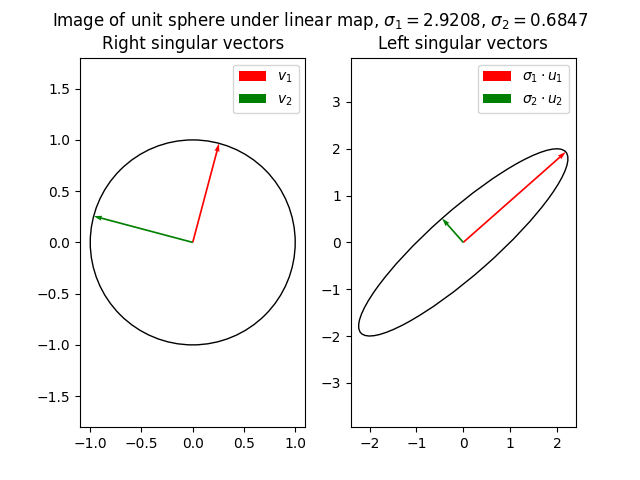
\includegraphics[width=0.7\textwidth]{eq37_plot_of_singular_vectors}
		\caption{Exercise 4.3: Plot of singular vectors of $A=\begin{bmatrix}
			1 & 2\\
			0 & 2
		\end{bmatrix}$ from Equation 3.7 in Example 3.1 of the book}
		\label{fig:4.3-eq3.7}
	\end{figure}
	\begin{figure}
		\centering
		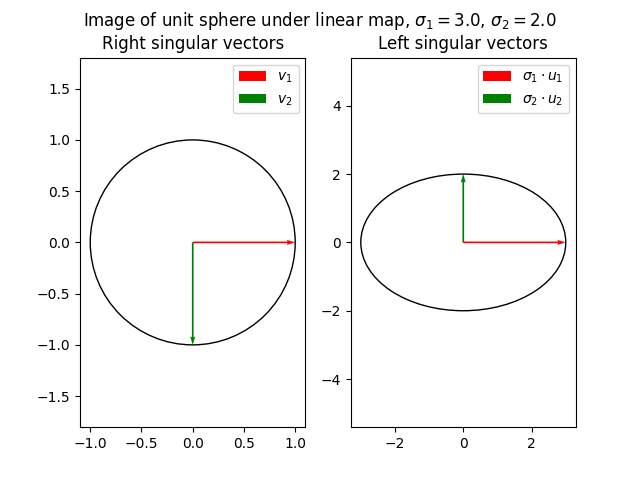
\includegraphics[width=0.7\textwidth]{a_plot_of_singular_vectors}
		\caption{Exercise 4.3a: Plot of singular vectors of $A=\begin{bmatrix}
				3 & 0\\
				0 & -2
			\end{bmatrix}$ from Exercise 4.1(a)}
		\label{fig:4.3a}
	\end{figure}
	\begin{figure}
		\centering
		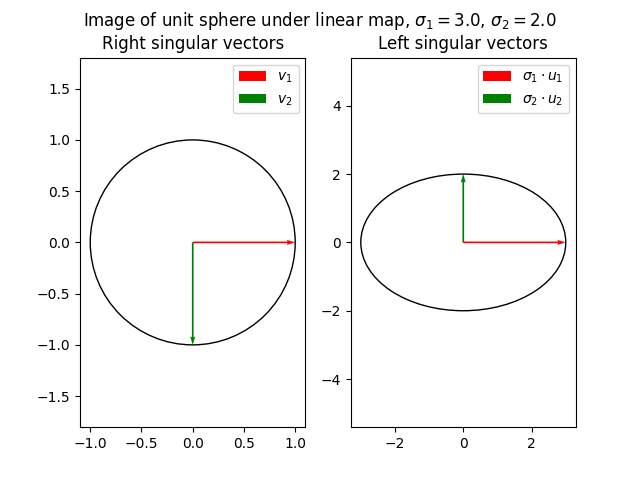
\includegraphics[width=0.7\textwidth]{a_plot_of_singular_vectors}
		\caption{Exercise 4.3(b): Plot of singular vectors of $A=\begin{bmatrix}
				2 & 0\\
				0 & -3
			\end{bmatrix}$ from Exercise 4.1(b)}
		\label{fig:4.3b}
	\end{figure}
	\begin{figure}
		\centering
		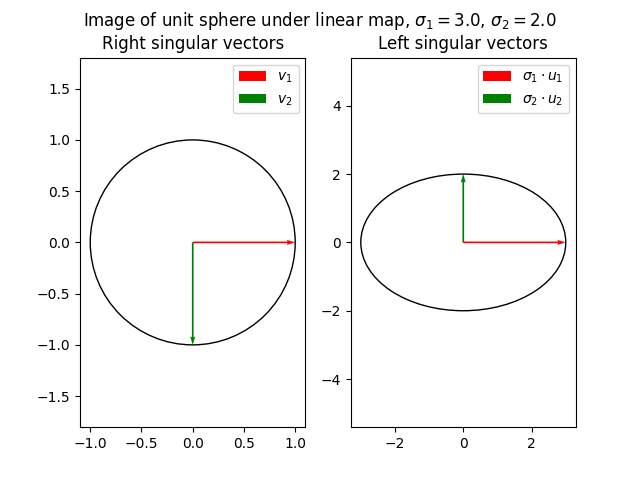
\includegraphics[width=0.7\textwidth]{a_plot_of_singular_vectors}
		\caption{Exercise 4.3(c): Plot of singular vectors of $A=\begin{bmatrix}
				0 & 2\\
				0 & 0\\
				0 & 0
			\end{bmatrix}$ from Exercise 4.1(c)}
		\label{fig:4.3c}
	\end{figure}
	\begin{figure}
		\centering
		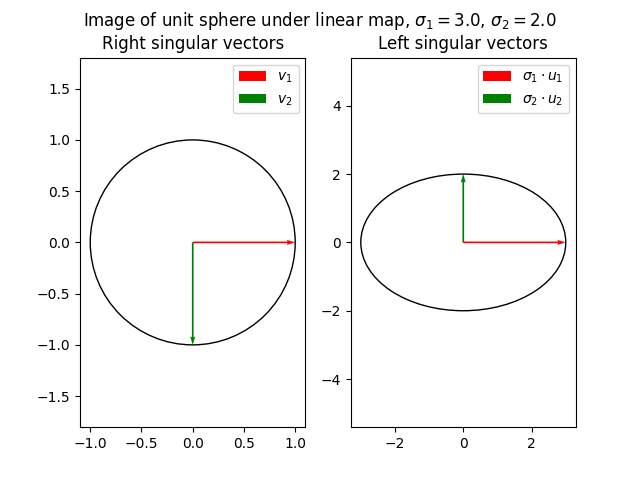
\includegraphics[width=0.7\textwidth]{a_plot_of_singular_vectors}
		\caption{Exercise 4.3(d): Plot of singular vectors of $A=\begin{bmatrix}
				1 & 1\\
				0 & 0
			\end{bmatrix}$ from Exercise 4.1(d)}
		\label{fig:4.3d}
	\end{figure}
	\begin{figure}
		\centering
		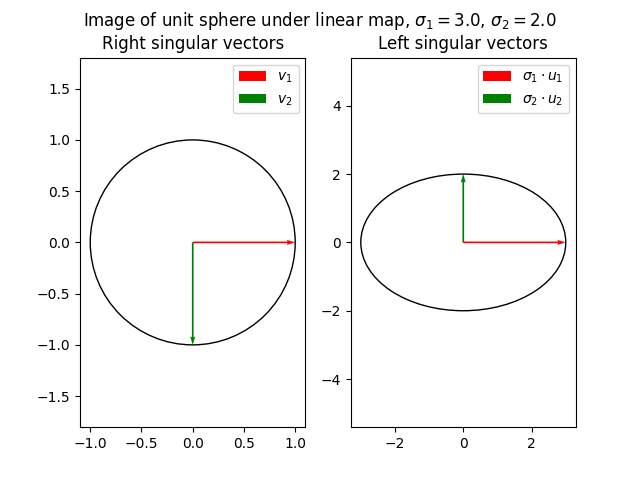
\includegraphics[width=0.7\textwidth]{a_plot_of_singular_vectors}
		\caption{Exercise 4.3: Plot of singular vectors of $A=\begin{bmatrix}
				1 & 1\\
				1 & 1
			\end{bmatrix}$ from Exercise 4.1(e)}
		\label{fig:4.3e}
	\end{figure}
\end{sol}

\begin{ex}{4.4}
	Two matrices $A,B\in\mathbb{C}^{m\times m}$ are \emph{unitarily equivalent} if $A=QBQ^*$ for
	some unitary $Q\in\mathbb{C}^{m\times m}$. Is it true or false that $A$ and $B$ are unitarily
	equivalent if and only if they have the same eigenvalues?
\end{ex}

\begin{sol}
	\
	This is true.
	\begin{proof}
		(``$\implies$"): Suppose that $A$ and $B$ are unitarily equivalent, meaning there is a unitary
		matrix $Q\in\mathbb{C}^{m\times m}$ such that $A=QBQ^*$. By Theorem 4.1, every matrix
		in $\mathbb{C}^{m\times m}$ has an SVD, so let $U,V$ be unitary matrices of the left and
		right singular vectors of $B$, and $\Sigma$ be the diagonal matrices consisting of the
		singular values of $B$, so that $B=U\Sigma V^*$, where $V^*$ denotes the adjoint of $V$
		(and hence its inverse since $V$ is unitary). Then
		\begin{align*}
			A &= QBQ^*\\
			A &= QU\Sigma V^*Q^*\\
			A &= (QU)\Sigma (QV)^*
		\end{align*}
		The product of two unitary matrices is unitary. To see this, note that if $x\in\mathbb{C}^m$, then
		\[
		\lVert QUx\rVert = \lVert Q(Ux)\rVert = \lVert Ux\rVert = \lVert x\rVert
		\]
		because both $Q$ and $U$ are unitary. Similarly $QV$ is unitary. Thus, the equation above for $A$
		is a singular value decomposition of $A$. By Theorem 4.1, the singular values of $A$ are uniquely
		determined, so the diagonal entries in $\Sigma$ must also be singular values of $A$.
		
		\
		(``$\impliedby$"): Suppose $A$ and $B$ have the singular values. Then their SVD consists of the same
		diagonal matrix $\Sigma$. Let $S,R,U,V$ be unitary matrices composing the SVDs of $A$ and $B$, respectively:
		\[
		A=S\Sigma R^*\quad B=U\Sigma V^*
		\]
		Then $\Sigma = U^*BV$, and hence
		\begin{align*}
			A=S(U^*BV)R^*=(SU^*)B(RV^*)^*
		\end{align*}
		Just like before the product of unitary matrices is unitary, so $A$ and $B$ are unitarily equivalent.
	\end{proof}
\end{sol}

\begin{ex}{4.5}
	Theorem 4.1 asserts that every $A\in\mathbb{C}^{m\times n}$ has an SVD $A=U\Sigma V^*$. Show that if $A$
	is real, then it has a real SVD ($U\in \mathbb{R}^{m\times m}$, $V\in\mathbb{R}^{n\times n}$).
\end{ex}

\begin{sol}
	\
	\begin{proof}
		Since $A\in\mathbb{R}^{m\times n}$, we can consider it also as a matrix over the vector space
		$\mathbb{C}^{m\times n}$. Thus $A$ has an SVD, with $U\in\mathbb{C}^{m\times m}$ and
		$V\in\mathbb{C}^{n\times n}$ unitary matrices, and $\Sigma\in\mathbb{R}^{m\times n}$ a diagonal
		matrix, since the singular values of $A$ are nonnegative real numbers. We have
		\begin{align*}
			A&=U\Sigma V^*\\
		\end{align*}
		Then $AV=U\Sigma$, so $Av_j=\sigma_j u_j$ for each $j$. If $v_j$ has complex entries, split it into
		real and imaginary parts as $v_j=\Re v_j + i\Im v_j$, and similarly $u_j=\Re u_j+i\Im u_j$. Then
		\begin{align*}
			A\Re v_j + iA\Im v_j = Av_j = \sigma_j u_j = \sigma_j \Re u_j + i \sigma_j \Im u_j
		\end{align*}
		Hence, since $A$ is real, we have
		\[
		A\Re v_j = \sigma_j \Re u_j\quad \quad A\Im v_j=\sigma_j \Im u_j
		\]
		Note that $A^*A=V\Sigma^2V^*$, so $A^*V=V\Sigma^2$. This implies that $A^*Av_j=\sigma_j^2v_j$ for each $j$,
		and hence
		\[
		A^*A\Re v_j = \sigma_j^2 \Re v_j,\quad A^*A\Im v_j = \sigma_j^2\Im v_j
		\]
		Since $v_j$ is an eigenvector, it is nonzero, so either $\Im v_j$ or $\Re v_j$ must be nonzero,
		and hence is an eigenvector. (Proof incomplete).
	\end{proof}
\end{sol}

\end{document}